\chapter{Numerical integration using interpolating polynomials}
% \Chapter{Numerical integration}{using interpolating polynomials}
\label{chap3}
In Chapter \ref{chap2} we derived the Rayleigh integral, whereas the goal of our thesis is to find algorithms that can compute the integral (whilst reducing error and being time-efficient).
To find these algorithms we first simplify the integral.
Afterwards we interpolate the integrand (or a part of it) by polynomials, which we can then integrate to approximate the simplified integral.
In the next chapter (Chapter \ref{chap4}) we extend these simplified methods to the Rayleigh integral and in Chapter \ref{chap5} we look at results from those methods.
This chapter thus forms a basis for the numerical integration methods used throughout this thesis.

First, we present the simplification of the Rayleigh integral (equation \ref{eq:rayleigh}):
\begin{tcolorbox}[sharp corners, colback=white]
    We consider an integral on the interval $[x_L, x_R]$, where we define $f: \mathbb R \to \mathbb R$, $g: \mathbb R \to \mathbb R$ with $f(x)=g(x)=0$ for $x\notin [x_L, x_R]$\footnote{We make this approximation (it is an approximation since the wavefield is small for large distances away from the source) due to limitations of our algorithms. Also, in reality, the wavefield for the pressure must be measured/sampled and for this only a finite grid of sensors is used (so for the pressure function this assumption is the best we can do).}
    and let $a \in \mathbb R$, the simplification is to evaluate the integral (which is a function of $a$)
    \vspace{-1em}
    \begin{equation}
        \int_{x_L}^{x_R} f(x) g(x+a) \mathrm d x \,. \label{eq:definite_int}
    \end{equation}
\end{tcolorbox}
Note that the Rayleigh integral (equation \ref{eq:rayleigh}) is also an integral over the product of two functions, that is, the derivative of Green's function and the function for the pressure at $z=0$, where the Green's function gets shifted after changing the prediction point $\mathbf r_A$ (this must be done repeatedly in seismic imaging since we need to propagate the wavefield from each layer to the subsequent, needing roughly the same grid of points where the pressure is known), which translates to changing the constant $a$ in the above integral.
To clarify, in the above integral $f(x)$ represents the pressure part of the Rayleigh integral and $g(x)$ represents the derivative of the Green's function.
We also note that the derivative of Green's function (and therefore $g(x)$ in our simplification) is known.

The first section of this chapter presents an algorithm based on separately interpolating the two parts of the integral (i.e. the known part $g(x)$ and the unknown part $f(x)$) before integrating, Subsection \ref{sep_interpol_3d} will continue on this subject.
The second section will focus on the derivation of a formula that evaluates the above integral by interpolating the product of the two parts, Subsection \ref{doub_alter} discusses the extension of this method to the Rayleigh integral.
Specifically, in the second section, we derive the $2$nd-order Newton-Cotes equation called Simpson's rule, afterwards we will discuss a more general version of this equation.
In the third and final section we present numerical examples for the evaluation of integrals using the methods from the previous two sections, which can be used as an example for future research planning to implement the methods for the evaluation of the Rayleigh integral.
Also, this is done to clarify the methods described.

Only basic methods of polynomial interpolation are discussed, mostly due to our main focus to approximate the above integral.
For more information on interpolatory methods the reader is referred to \citeauthor{integration} \cite{integration} and \citeauthor{Book_Kees} \cite[Chapter 2]{Book_Kees}.


\section{Separate interpolation}
\label{sep_interpol}
To approximate the simplified integral in equation \ref{eq:definite_int}, we will interpolate the functions $f(x)$ and $g(x)$ separately.

To achieve this, the interval $[x_L,x_R]$ is first partitioned into $\ell$ equally large subintervals $[x_0, x_1]$, $[x_1, x_2]$, \dots, $[x_{\ell-1}, x_\ell]$. That is, $x_1 - x_0 = x_2 - x_1 = \cdots = x_\ell - x_{\ell-1}$ and $x_L = x_0$ and $x_R = x_\ell$. Because we are integrating, closed and open intervals are not distinguished and are therefore always denoted as closed intervals.

For each interval $[x_i, x_{i+1}]$ with $0 \leq i \leq \ell -1$ both function are interpolated by polynomials, in Section \ref{box:newton_pol} there is a simple method to achieve this, but other methods like spline interpolation \cite[Section 2.5]{Book_Kees} can also be used. We write
\begin{equation}
    f_{i}(x) = \sum_{j=0}^{n_f} b_{ij} x^j \,,  \quad
    g_{i}(x) = \sum_{k=0}^{n_g} c_{ik} x^k \nonumber
\end{equation}
for each interval $[x_i, x_{i+1}]$ where $f_i(x)$ and $g_i(x)$ are polynomials of degree at most $n_f$th and $n_g$th, respectively.
Using the fact that the intervals are equidistant the interpolation can be achieved with a time complexity of $\mathcal O(n_f^2 \ell + n_g^2 \ell)$ \cite{pol_inter}.
Furthermore, since we need to store all values of $b_{ij}$ and $c_{ik}$ the space complexity is $\mathcal O(n_f\ell + n_g\ell)$.

We assume the prediction points (the points corresponding to different values of $a$ in equation \ref{eq:definite_int}) are spaced equidistantly (this is often the case).
Therefore, we let $a$ be a multiple of the interval width $(x_1 - x_0)$, we can assume this because the integral width was previously arbitrary.
Provided that we write $a = m (x_1 - x_0)$ with $m \in \mathbb N$ and $0\leq m \leq s$, where $s$ denotes the number of prediction points (i.e. the number of sensors), the integral in equation \ref{eq:definite_int} becomes (remember that $f(x)=g(x)=0$ for $x \notin [x_L, x_R]$)
\begin{align}
    \int_{x_L}^{x_R} f(x') g(x'+a) \mathrm d x' &= \int_{x_L-a}^{x_R-a} f(x-a) g(x) \mathrm d x \nonumber \\
                                                &\approx \sum_{i=0}^{\ell-m} \int_{x_i}^{x_{i+1}} f_{i}(x-a) g_{i}(x) \mathrm d x \nonumber \\
                                                &= \sum_{i=0}^{\ell-m} \int_{x_i}^{x_{i+1}} f_{i+m}(x) g_{i}(x) \mathrm d x \nonumber \\
                                   &= \sum_{i=0}^{\ell-m} \int_{x_i}^{x_{i+1}} \sum_{j=0}^{n_f} \sum_{k=0}^{n_g} b_{i+m,j} c_{ik} x^{j+k} \mathrm d x \nonumber \\
                                   &= \sum_{i=0}^{\ell-m} \sum_{j=0}^{n_f} \sum_{k=0}^{n_g} b_{i+m,j} c_{ik} \int_{x_i}^{x_{i+1}} x^{j+k} \mathrm d x \nonumber \\
                                   &= \sum_{i=0}^{\ell-m} \sum_{j=0}^{n_f} b_{i+m,j} \sum_{k=0}^{n_g} c_{ik} \frac{x_{i+1}^{j+k+1} - x_i^{j+k+1}}{j+k+1} \,. \label{eq:sums_int}
\end{align}
Storing the values of
\begin{equation}
    d_{ij} = \sum_{k=0}^{n_g} c_{ik} \frac{x_{i+1}^{j+k+1} - x_i^{j+k+1}}{j+k+1} \,, \label{eq:calc_dij}
\end{equation}
for all $i$ and $j$ then allows us to rewrite equation \ref{eq:sums_int}, giving
\begin{equation}
    \int_{x_L}^{x_R} f(x) g(x+a) \mathrm d x \approx \sum_{i=0}^{\ell-m} \sum_{j=0}^{n_f} b_{i+m,j} d_{ij} \,. \label{eq:final_int}
\end{equation}
After storing the values of $(x_{i+1}^{j+k+1} - x_i^{j+k+1})/(j+k+1)$ for all $j+k$ and $i$ with a space and time complexity of $\mathcal O(n_f\ell + n_g\ell)$, we can calculate the values of $d_{ij}$ with a time complexity of $\mathcal O(n_f n_g \ell)$ and a space complexity of $\mathcal O(n_f \ell)$.

To compute the space and time complexity of approximating the integral, we note that initializing this algorithm can be done in $\mathcal O((n_f+n_g)^2 \ell)$ time and $\mathcal O(n_f\ell + n_g\ell)$ space.
The algorithm would then step through all the prediction points $s$, calculating the sum in equation \ref{eq:final_int}, having an overall time complexity of $\mathcal O(n_f \ell s)$ and a total space complexity of $\mathcal O(n_f \ell + n_g \ell + s)$ since we need to store the results as well.

Note that the final time complexity is independent of $n_g$. Since the (derivative of) Green's function is known, we could interpolate it by using a polynomial of a high degree. This is an important result as we can make use of it to improve the accuracy of our approximation.
Also, we can increase the domain on which we interpolate the derivative of Green's function, reducing the approximation made in the simplified version of the Rayleigh integral.


\section{Combined interpolation}
\label{comb_interpol}
In this section we present another method of finding the integral in equation \ref{eq:definite_int}, the method relies on interpolating the product of the functions $f(x)$ and $g(x)$.

The method is based on the Newton-Cotes equations and implementing these equations is generally simple. Furthermore, by using this method, we can reduce the space complexity compared to the method in Section \ref{sep_interpol}. However, in some situations we present in Section \ref{examples} and Chapter \ref{chap5} the accuracy of this method is lacking.
Nevertheless, this method still provides a cornerstone for one of the two methods used to evaluate an artificial Rayleigh integral in Chapter \ref{chap5}.

In the first subsection we derive the $2$nd-order Newton-Cotes equation commonly known as Simpson's rule, the derivation, however, requires knowledge of interpolating with polynomials, for which Newton polynomials are used.
In the next subsection we discuss the generalization of the Newton-Cotes equations, which can be described by the Cotesian numbers.
Then, we present a method to go from the (generalized) equations to approximating integrals, where we introduce notation that will also be used in following chapters.

\subsection{Derivation of Simpson's rule}
\label{derivation_simpson}
To derive the $2$nd-order Newton-Cotes equation named Simpson's rule, we first need to be able to interpolate $3$ points by a parabola (or a polynomial of lower order).
Below we present the general method of Newton polynomials that allows us to interpolate $n+1$ points by a polynomial.

\begin{tcolorbox}[enhanced, size=fbox, shadow={2mm}{-2mm}{0mm}{gray!30!white}, boxrule={1.5pt}, colback=white, sharp corners, breakable, boxsep=5pt, left=2pt, right=2pt, title=\Large{Newton Polynomials}]
    \label{box:newton_pol}
    \textbf{\Large{Theorem}}

    Let $f: \mathbb R \to \mathbb R$ denote the function that we want to interpolate on the points $x_0, x_1, \dots, x_n$.
    For compacter notation we write $f_i$ instead of $f(x_i)$ from now on\footnote{The notation is adapted from \citeauthor{newton_pol} \cite{newton_pol}.}.

    After writing
    \begin{equation}
        \begin{matrix}
            x_0 & f_0 \\
                & & \frac{f_1-f_0}{x_1-x_0} \\
            x_1 & f_1 & & \frac{\frac{f_2-f_1}{x_2-x_1} - \frac{f_1-f_0}{x_1-x_0}}{x_2-x_0} \\
                & & \frac{f_2-f_1}{x_2-x_1} & & \ddots \\
            x_2 & f_2 & & \vdots\\
                &  & \vdots & & \Rdots \\
            \vdots & \vdots & & \cdots \\
                   &        & \frac{f_n-f_{n-1}}{x_n-x_{n-1}} \\
            x_n & f_n
        \end{matrix} \label{eq:newton_pol}
    \end{equation}
    the top row read from left to right form the constants of the interpolating polynomials.
    That is, the interpolating polynomial $p(x)$ is given by:

    \begin{equation}
        p(x) = f_0 + \frac{f_1-f_0}{x_1-x_0} (x-x_0) + \frac{\frac{f_1-f_0}{x_1-x_0} - \frac{f_2-f_1}{x_2-x_1}}{x_2-x_0} (x-x_0) (x-x_1) + \cdots \,.\label{eq:newton_pol_func}
    \end{equation}

    \vspace{.5em}
    \hrule
    \hrule
    \vspace{.5em}

    \textbf{\Large{Proof:}}
    We will prove this result by using induction on the number of points $n$ we interpolate. The induction base with $n=1$ is easily verified, as the interpolating polynomial is just the horizontal line $p(x)=f_0$. For the induction hypothesis we assume that we can interpolate $n$ points by constructing a Newton polynomial according to the recurrence relation in equation \ref{eq:newton_pol}, we now seek to prove that we can interpolate $n+1$ points whilst still using the same recurrence to determine all coefficients.

    Let $p$ interpolate $f$ at $\{ x_0, x_1, \dots, x_{n-1} \}$ and let $q$ interpolate $f$ at $\{ x_1, x_2, \dots, x_{n}\}$, which is possible due to the induction hypothesis. Also, denote the coefficient of $x^{n-1}$ in $p$ and $q$ by $p_{n-1}$ and $q_{n-1}$, respectively.
    We define
    \begin{equation}
        r(x) = \frac{(x-x_0)q(x) + (x_{n}-x)p(x)}{x_{n}-x_0} \nonumber
    \end{equation}
    and note that $r(x_i) = f(x_i)$ for $i \in \{ 0, 1, \dots, n \}$. Also, the coefficient of $x^{n}$ in $r$ is given by $(q_{n-1} - p_{n-1})/{(x_{n}-x_0)}$, following the recurrence relation in equation \ref{eq:newton_pol} (note that the other coefficients are the same as those of $p$ and thus can be computed using the same relation). Thus, we have shown the induction step, proving the theorem.

    \vspace{.5em}
    \hrule
    \hrule
    \vspace{.5em}

    \textbf{\Large{Example}}

    Let us say that we want to interpolate the following points $(1, \frac{5}{4}), (\frac{8}{5}, -\frac{4}{5}), (3, \frac{7}{2}) (\frac{7}{2}, 3)$ with a polynomial.
    We first construct the same triangle as in equation \ref{eq:newton_pol} with the above coordinates:
    \begin{equation}
        \begin{matrix}
            x_0 = 1 & f_0 = \frac{5}{4} \\
                & & \frac{-\frac{4}{5}-\frac{5}{4}}{\frac{8}{5}-1} = -\frac{41}{12} \\
            x_1 = \frac{8}{5} & f_1 = -\frac{4}{5} & & \frac{\frac{43}{14} + \frac{41}{12}}{3-1} = \frac{545}{168} \\
                & & \frac{\frac{7}{2}+\frac{4}{5}}{3-\frac{8}{5}} = \frac{43}{14} & & \frac{-\frac{15}{7} - \frac{545}{168}}{\frac{7}{2}-1} = -\frac{181}{84} \,. \\
            x_2 = 3 & f_2 = \frac{7}{2} & & \frac{-1 - \frac{43}{14}}{\frac{7}{2}-\frac{8}{5}} = -\frac{15}{7} \\
                   &        & \frac{3-\frac{7}{2}}{\frac{7}{2}-3} = -1 \\
            x_3 = \frac{7}{2} & f_3 = 3
        \end{matrix}
        \nonumber
    \end{equation}
    After inserting the coefficients in equation \ref{eq:newton_pol_func} we obtain the formula for the interpolating polynomial:
    \begin{equation}
        p(x) = \frac{5}{4} - \frac{41}{12} (x-1) + \frac{545}{168} (x-1)(x-\frac{8}{5}) - \frac{181}{84} (x-1)(x-\frac{8}{5})(x-3) \,. \label{eq:newton_pol_fun_values}
    \end{equation}

    The figure below illustrates that the above formula (equation \ref{eq:newton_pol_fun_values}) indeed interpolates the points.
    \begin{figure}[H]
        \vspace{-2em}
        \centering
        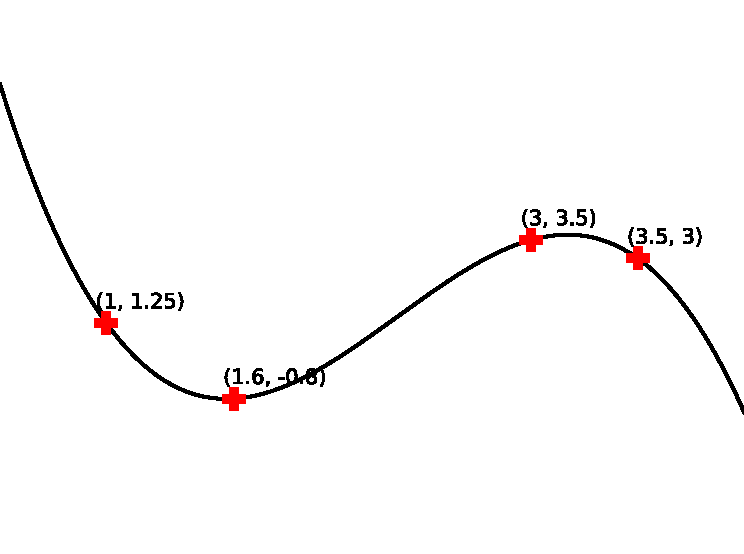
\includegraphics[width=.5\textwidth]{pictures/newton_polynomial}
        \vspace{-1em}
    \end{figure}

\end{tcolorbox}

Let us now derive Simpson's rule. We define three equally spaced points (with step size $h$) and denote them as $x_0$, $x_1=x_0+h$ and $x_2=x_0+2h$ and their corresponding function values by $f_0$, $f_1$ and $f_2$, respectively. To form the Newton polynomial, we first write the points in the form of equation \ref{eq:newton_pol}:
\begin{equation}
    \begin{matrix}
        x_0 & f_0 \\
            & & \frac{f_1-f_0}{h} \\
        x_1 & f_1 & & \frac{f_0 + f_2-2f_1}{2h^2} \\
            & & \frac{f_2-f_1}{h} \\
        x_2 & f_2 \\
    \end{matrix} \,.\nonumber
\end{equation}
The interpolating polynomial then becomes
\begin{equation}
    p(x) = f_0 + \frac{f_1-f_0}{h} (x-x_0) + \frac{f_0 + f_2-2f_1}{2h^2} (x-x_0)(x-x_1) \,.\nonumber
\end{equation}
Integrating from $x_0$ to $x_2$ (keeping in mind that $x_1-x_0 = h$ and $x_2-x_0 = 2h$) now gives us Simpson's rule:
\begin{align}
    \int_{x_0}^{x_2} p(x) \mathrm dx &= \left[f_0 x + \frac{f_1-f_0}{2h} (x-x_0)^2 + \frac{f_0 + f_2-2f_1}{2h^2} \left(\frac{x^3}{3}-(x_0+x_1)\frac{x^2}{2} + x_0 x_1 x\right)\right]_{x_0}^{x_2} \nonumber \\
                                     &= 2hf_0 + 2h(f_1-f_0) + \frac{f_0 + f_2-2f_1}{2h^2} \left(\frac{x_2^3-x_0^3}{3}-(x_0+x_1)\frac{x_2^2-x_0^2}{2} + 2h x_0 x_1 \right) \nonumber \\
                                     &= 2hf_1 + \frac{f_0 + f_2-2f_1}{2h^2} \left(\frac{8h^3}{3}+2x_0^2h+4x_0h^2-(2h^2+2hx_0)(2x_0+h) + 2h x_0 (x_0+h) \right) \nonumber \\
                                     &= 2hf_1 + \frac{f_0 + f_2-2f_1}{2h^2} \left(\frac{2h^3}{3}+4x_0^2h+2x_0h^2-2hx_0(2x_0+h)  \right) \nonumber \\
                                     &= 2hf_1 + \frac{f_0 + f_2-2f_1}{2h^2} \frac{2h^3}{3} \nonumber \\
                                     &= 2hf_1 + \frac{h}{3}(f_0 + f_2-2f_1) \nonumber \\
                                     &= \frac{h}{3}(f_0 + 4f_1 + f_2) \,.\nonumber
\end{align}
In Subsection \ref{newton_cotes_integrals} we explain how one can use this result to approximate integrals, together these section form the basis for the combined interpolation method in Chapter \ref{chap4}.

\subsection{Cotesian numbers}
\label{sec:cotesian}
Instead of interpolating $3$ points by a parabola, we can also interpolate $n+1$ points by an $n$th-order polynomial (we note that the order can be lower than $n$), by doing this, we obtain the Cotesian numbers used in Newton-Cotes equations.
Higher order equations can be more accurate in approximating integrals than Simpson's rule.

We will denote the Cotesian numbers as $c_0$, $c_1$, $\dots$, $c_n$, which are defined such that after defining points $x_0$, $x_1$, \dots, $x_n$ and function values $f_0$, $f_1$, $\dots$, $f_n$ the integral over the interpolated polynomial can be approximated by $h(c_0f_0+c_1f_1+\cdots+c_nf_n)$, where $h$ is the distance between two points $x_i$ and $x_{i+1}$.

To calculate the Cotesian numbers, we can solve the following system of equations (the proof of this statement is in Appendix \ref{app:proofs} as the proof of Theorem \ref{theorem:mat}):
\begin{equation}
    \begin{bmatrix}
        1&0&0&\cdots&0 \\
        1&1&1&\cdots&1 \\
        1&2&2^2&\cdots&2^n \\
        \vdots&\vdots & \vdots & \ddots & \vdots\\
        1&n&n^2&\cdots&n^n
    \end{bmatrix}^\top
    \begin{bmatrix}
        c_0\\
        c_1\\
        c_2\\
        \vdots \\
        c_n
    \end{bmatrix}
    =
    \begin{bmatrix}
        n/1 \\
        n^2/2 \\
        n^3/3 \\
        \vdots \\
        n^{n+1}/(n+1)
    \end{bmatrix} \,,\nonumber
\end{equation}
where the matrix on the left-hand side is the Vandermonde matrix.
Since the inverse of the Vandermonde matrix exists in closed form (see Lemma \ref{lemma:invertible} in Appendix \ref{app:proofs}), the matrix can be brought to the other side \cite{vandermonde_inv}.
After denoting the signed Stirling numbers of the first kind as $s(n, k)$ and doing just that we get a non-recursive formula for the coefficients $c_i$ for $0 \leq i \leq n$ (Theorem \ref{theorem:calc} in Appendix \ref{app:proofs}):
\begin{equation}
    c_i = \frac{1}{(n-1)!} \binom{n}{i} \sum_{j=0}^{n} \sum_{m=0}^{n-j} i^m n^{j} \frac{(-1)^{i+n} s(n+1, j+m+1) }{j+1} \,. \nonumber
\end{equation}
% \begin{equation}
%     c_i =
%     \begin{dcases}
%         \frac{1}{(n-1)!}\sum\limits_{k=1}^{n} \frac{n^k s(n, k)}{k+1} & i = 0 \text{ or } i=n\\
%         \frac{1}{(n-1)!}\binom{n}{i}\sum\limits_{j=1}^{i} \sum\limits_{k=1}^{n-i} n^{j+k} \frac{s(i, j)s(n-i, k)}{(k+1)\binom{j+k+1}{k+1}} & \text{otherwise}
%     \end{dcases}\nonumber
% \end{equation}
For simplicity, one can also look these numbers up, since they constitute a sequence in the OEIS (the On-Line Encyclopedia of Integer Sequences, \url{http://oeis.org/}). In terms of these sequences\footnote{For the corresponding sequences we refer the reader to OEIS Foundation Inc. (2022), Denominators of Cotesian numbers, Entry \href{http://oeis.org/A002176}{A002176} and Numerators of Cotesian numbers, Entry \href{http://oeis.org/A100642}{A100642} in The On-Line Encyclopedia of Integer Sequences, \url{http://oeis.org/A002176} and \url{http://oeis.org/A100642}.} we can write the Cotesian numbers as:
\begin{equation}
    \frac{nh}{\textrm{A002176}(n)} \left[\sum_{i=0}^n \textrm{A100642}\left(\frac{n(n+1)}{2} + i\right)f_i \right] \,. \nonumber
\end{equation}
The Cotesian numbers then determine the Newton-Cotes equations that can be used for approximating integrals:
\begin{gather}
    \frac{h}{2}(f_0 + f_1) \nonumber \\
    \frac{h}{3}(f_0+4f_1+f_2) \nonumber \\
    \frac{3h}{8}(f_0 + 3f_1 + 3f_2 + f_3) \nonumber \\
    \frac{2h}{45}(7f_0 + 32f_1 + 12f_2 + 32f_3 + 7f_4) \nonumber \\
    \frac{5h}{288}(19f_0 + 75f_1 + 50f_2 + 50f_3 + 75f_4 + 19f_5) \nonumber \\
    \frac{h}{140}(41f_0 + 216f_1 + 27f_2 + 272f_3 + 27f_4 + 216f_5 + 41f_6) \nonumber \\
    \frac{7h}{17280}(751f_0 + 3577f_1 + 1323f_2 + 2989f_3 + 2989f_4 + 1323f_5 + 3577f_6 + 751f_7) \,. \nonumber \\
    \udots \hspace{5em} \vdots \hspace{5em} \vdots \hspace{5em} \vdots \hspace{5em} \ddots \label{eq:newton_cotes}
    % & \frac{4h}{14175}(989f_0 + 5888f_1 - 928f_2 + 10496f_3 - 4540f_4 + 10496f_5 - 928f_6 + 5888f_7 + 989f_8) \nonumber \\
    % & \frac{9h}{89600}(2857f_0 + 15741f_1 + 1080f_2 + 19344f_3 + 5778f_4 + 5778f_5 + 19344f_6 + 1080f_7 + 15741f_8 + 2857f_9) \nonumber \\
    % & \frac{5h}{299376}(16067f_0 + 106300f_1 - 48525f_2 + 272400f_3 - 260550f_4 + 427368f_5 - 260550f_6 + 272400f_7 - 48525f_8 + 106300f_9 + 16067f_{10}) \nonumber \\
    % & \frac{11h}{87091200}(2171465f_0 + 13486539f_1 - 3237113f_2 + 25226685f_3 - 9595542f_4 + 15493566f_5 + 15493566f_6 - 9595542f_7 + 25226685f_8 - 3237113f_9 + 13486539f_{10} + 2171465f_{11}) \nonumber \\
    % & \frac{h}{5255250}(1364651f_0 + 9903168f_1 - 7587864f_2 + 35725120f_3 - 51491295f_4 + 87516288f_5 - 87797136f_6 + 87516288f_7 - 51491295f_8 + 35725120f_9 - 7587864f_{10} + 9903168f_{11} + 1364651f_{12}) \nonumber \\
    % & \frac{13h}{402361344000}(8181904909f_0 + 56280729661f_1 - 31268252574f_2 + 156074417954f_3 - 151659573325f_4 + 206683437987f_5 - 43111992612f_6 - 43111992612f_7 + 206683437987f_8 - 151659573325f_9 + 156074417954f_{10} - 31268252574f_{11} + 56280729661f_{12} + 8181904909f_{13}) \nonumber \\
    % & \frac{7h}{2501928000}(90241897(f_0+f_{14}) + 710986864(f_1+f_{13}) - 770720657(f_2+f_{12}) + 3501442784(f_3+f_{11}) - 6625093363(f_4+f_{10}) + 12630121616(f_5+f_9) - 16802270373(f_6+f_8) + 19534438464f_7) \nonumber
\end{gather}
More information on this subject is only referenced \cite{cotesian1, cotesian2}.


\subsection{From Newton-Cotes equations to integrals}
\label{newton_cotes_integrals}
We now give the method for extending the Newton-Cotes equations to evaluate integrals.
Let us integrate over the interval $[x_L, x_R]$.
Partitioning this interval into the subintervals $[x_0, x_1]$, \dots, $[x_i, x_{i+1}]$, \dots $[x_{\ell-1}, x_{\ell}]$ with $x_0 = x_L$ and $x_\ell = x_R$, whilst noting that the subintervals do not have to be equidistant, allows us to approximate the integral over each subinterval by applying an $n$th-order Newton-Cotes equation (note that the order is allowed change for different subintervals) to that subinterval by defining the function values to be $f_0=f(x_i)$, $f_1 = f(x_i+\frac{x_{i+1}-x_i}{n})$, \dots, $f_k = f(x_i + k\frac{x_{i+1}-x_i}{n})$ \dots, $f_n = f(x_{i+1})$.

If we partition the original interval $[x_L, x_R]$ into equidistant subintervals and always apply Simpson's rule to the subinterval, we get the same effect as the following equation (where we evaluated the function at points $x_0, \dots, x_n$ with $x_0=x_L$ and $x_n = x_R$)
\begin{equation}
    \int_{x_L}^{x_R} f(x) \mathrm d x \approx \frac{h}{3}(f_0 + 4 f_1 + 2 f_2 + 4f_3 + \dots + 2 f_{n-2} + 4 f_{n-1} + f_n) \,.\nonumber
\end{equation}
This way, between every $3$ points $f_{2i}, f_{2i+1}, f_{2i+2}$ we interpolate the points by a parabola, integrate the parabola from $x_{2i}$ to $x_{2i+2}$, and we add up the results to approximate our integral.

Provided that we can split up the subintervals into the number of equidistant parts needed for the Newton-Cotes equations, we can also use vector notation to approximate the integral, for the above example this works out to be
\begin{equation}
    \int_{x_L}^{x_R} f(x) \mathrm d x \approx \mathbf c\mathbf f^\top \,,\nonumber
\end{equation}
with
\begin{equation}
    \mathbf c = \frac{h}{3}\begin{bmatrix}1&4&2&4&\dots&2&4&1\end{bmatrix}\quad \textrm{and} \quad
    \mathbf f = \begin{bmatrix}f_0&f_1&\dots&f_n\end{bmatrix} \,. \label{eq:vectors}
\end{equation}


\section{Examples}
\label{examples}
In this section we give numerical examples of approximating integrals using the methods described in previous sections of this chapter.
The examples provide an overview of the described methods and give an idea of what their accuracy is and where we can find room for improvement.
This section can also function as a tool to check the implementation of other researchers wanting to implement these methods themselves (note that the code to our implementation can be found in Appendix \ref{app:code}).

We start by interpolating functions using various types of polynomials.
The first type is $N_1$, the 1st-order Newton-Cotes equation known as the trapezoidal rule (this uses linear interpolation) for which the integral can be found at the top in equation \ref{eq:newton_cotes}.
This type is currently most commonly used for evaluating the Rayleigh integral and is therefore added as a benchmark.
The second type is $N_2$, the 2nd-order Newton-Cotes equation known as Simpson's rule.
The third type is $S_3$, a cubic spline interpolation.
Results of the interpolation can be seen in Figure \ref{fig:res_1}.
\begin{figure}[H]
    \vspace{-.5em}
    \begin{tabular}{rl}
        \subcaptionbox{\centering Interpolation of $h_1(x)$.}{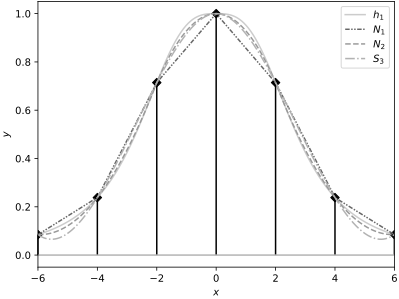
\includegraphics[width=.46\textwidth]{pictures/interpolate_func1}} &
        \subcaptionbox{\centering Interpolation of $h_2(x)$.\label{fig:res_1b}}{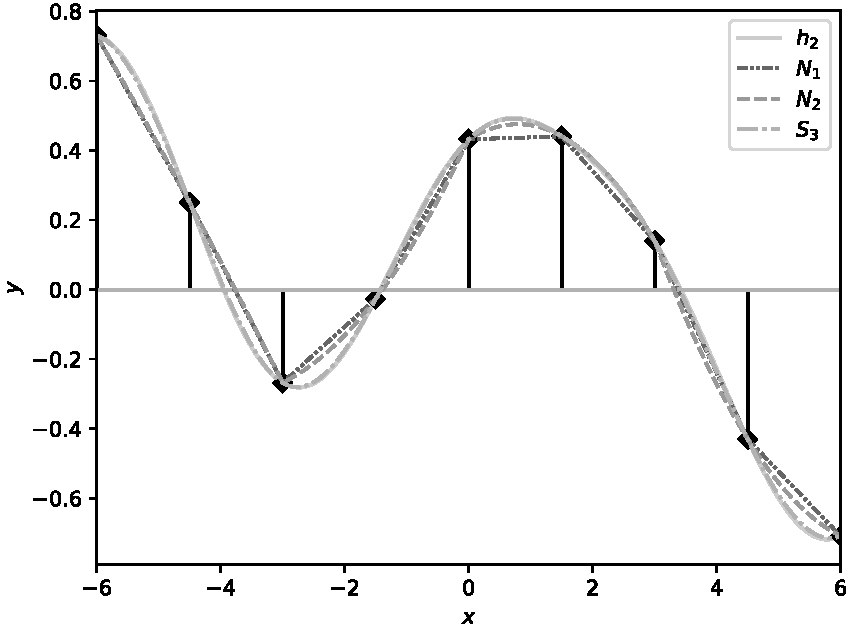
\includegraphics[width=.47\textwidth]{pictures/interpolate_func2}} \\
        \subcaptionbox{\centering Difference between interpolated functions and $h_1(x)$.\label{fig:diff_c}}{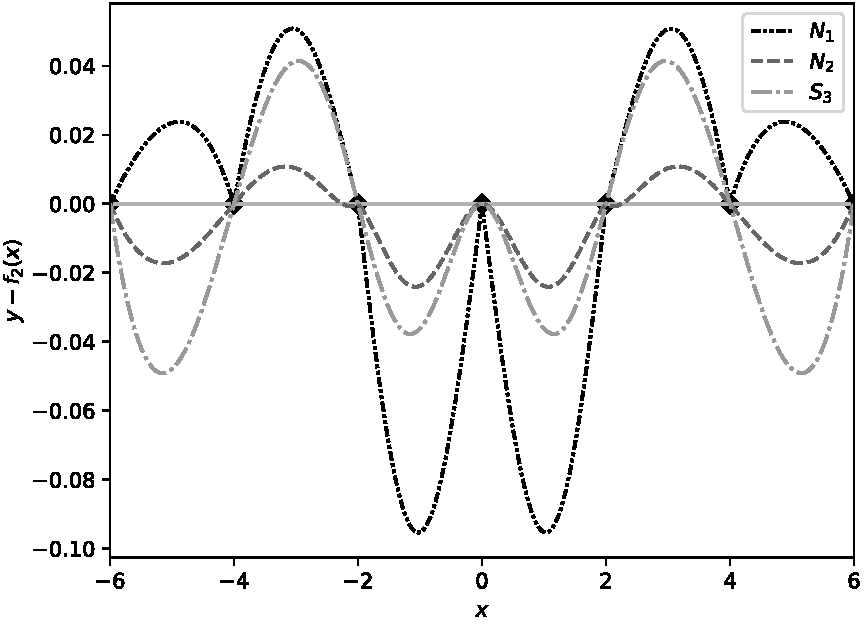
\includegraphics[width=.47\textwidth]{pictures/difference_func1}} &
        \subcaptionbox{\centering Difference between interpolated functions and $h_2(x)$.}{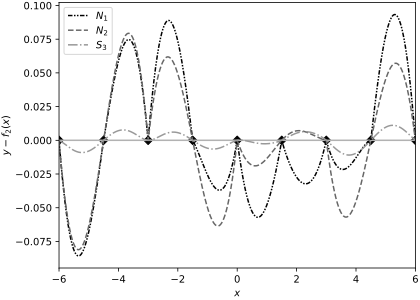
\includegraphics[width=.47\textwidth]{pictures/difference_func2}}
    \end{tabular}
    \vspace{-.2em}
    \caption{Interpolation of $h_1(x) = 1/(1+|x|^3/20)$ and $h_2(x) = \cos(\sqrt{(x-1)^2/4+1}) \cdot \sin(\sqrt{(x-2)^2/4+1})$ using $7$ and $9$ sample points of the function, respectively.}
    \label{fig:res_1}
    \vspace{-.8em}
\end{figure}
The integrals over the various interpolation types are listed in Table \ref{tab:res_1}, where a few are calculated explicitly later on in this section.
To illustrate how polynomials of higher order behave we have added a fourth type: $N_6$ (and the type $N_{1-6-1}$, which is the same as $N_6$ enclosed by two $N_1$'s to account for the number of sample points), being the 6th-order Newton-Cotes equation.

From Table \ref{tab:res_1} and Figure \ref{fig:res_1} we can see that $N_1$ got lucky with good approximation for the integral over function $h_1(x)$, since although $N_1(x) - h_1(x)$ (Figure \ref{fig:diff_c}) has the greatest deflections the resulting integral is very close to the actual integral because the average deflection is coincidentally close to zero.
However, with the other function ($h_2(x)$) the interpolation is less lucky, as other methods now give significantly better approximation to the integral.
\begin{table}[H]
    \vspace{-0.5em}
    \centering
    \begin{tabular}{p{.47\textwidth}p{.47\textwidth}}
        \begin{tabular}{cccc}
            Func. & Integral & Abs. diff. & Rel. diff. \\
            \hline
            $h_1(x)$ & $6.02845$ & - & - \\
            $N_1$    & $5.97902$ & $0.04943$ & $0.820\%$ \\
            $N_2$    & $5.95426$ & $0.07419$ & $1.23\%$ \\
            $N_6$    & $6.00540$ & $0.02305$ & $0.382\%$ \\
            $S_3$    & $5.92113$ & $0.10732$ & $1.78\%$
        \end{tabular} &
        \begin{tabular}{cccc}
            Func. & Integral & Abs. diff. & Rel. diff. \\
            \hline
            $h_2(x)$ & $0.79728$ & - & - \\
            $N_1$    & $0.82342$ & $0.02615$ & $3.28\%$ \\
            $N_2$    & $0.78280$ & $0.01448$ & $1.82\%$ \\
            $N_{1-6-1}$ & $0.88535$ & $0.08807$ & $11.0\%$ \\
            $S_3$    & $0.79930$ & $0.00203$ & $0.254\%$
        \end{tabular}
    \end{tabular}
    \vspace{-.2em}
    \caption{Various interpolations of function $h_1(x)$ on the left side and $h_2(x)$ on the right side together with the absolute difference and the relative difference between the integral and the correct integral.}
    \label{tab:res_1}
    \vspace{-0.5em}
    \centering
\end{table}
The large error in the approximation using $N_{1-6-1}$ is due to the boundaries of $N_6$.
These have great deflections causing an inaccurate result.
A method to remove the error would be to derive the coefficients using the integral, but instead of integrating over the full interval we can integrate over a subsection of it.
For the 6th-order Newton-Cotes equation we can take the integral from $x_1$ to $x_5$, resulting in the following formula (the original one can be found in equation \ref{eq:newton_cotes}):
\begin{equation}
   \frac{2h}{945}(-4f_0 + 171f_1 + 612f_2 + 332f_3 + 612f_4 + 171f_5 - 4f_6) \,. \label{eq:6star}
\end{equation}
We can then evaluate the integral of $h_2(x)$ again with an $N_{2-6^*-2}$ interpolation (we need to pad with two $N_2$'s since the new $N_{6^*}$ is integrated over fewer points), also we note that in the above formula the endpoints ($f_0$ and $f_6$) are weighted less since they do not directly contribute to the integral, only indirectly by interpolation.
The approximation for the integral becomes 0.77928, with an absolute difference of 0.01800 and a relative difference of 2.26\%.
This is a huge improvement compared to the relative error of 11.0\% from using $N_{1-6-1}$.
However, we do not investigate these methods further as the method still performes worse than $N_2$ and $S_3$ (this is instead left to future research in Section \ref{discussion}) and only polynomials up to the 2nd-order are used hereafter.

The best methods from above are therefore $N_2$ and $S_3$, however, since this is still combined interpolation (Section \ref{comb_interpol}) the integrals can also be approximated using separate interpolation (Section \ref{sep_interpol}).

We compare the combined interpolation using $S_3$ (thus we interpolate $f(x)\cdot g(x)$ by a cubic spline) and the separate interpolation using $S_3$ (thus we interpolate $f(x)$ and $g(x)$ separately where we interpolate $f(x)$ by a cubic spline and $g(x)$ to a high degree since it is known and combine the results by the method described in Section \ref{sep_interpol}).
The difference between the functions and their interpolations can be seen in Figure \ref{fig:res_2}, where we note that $h_2(x) = f_2(x)\cdot g_2(x)$ but that $h_1(x) \neq f_1(x)\cdot g_1(x)$ due to the function that was chosen.
The corresponding differences are listed in Table \ref{tab:res_2}, and the calculation of $S_3$ -- S can be found at the end of this section.
\begin{table}[H]
    \centering
    \begin{tabular}{p{.4\textwidth}p{.4\textwidth}}
        % \subcaptionbox{hihi}{\begin{tabular}{r} hi \\ hi \end{tabular}}
        % \subcaptionbox{hihi}{\begin{tabular}{r} hi \\ hi \end{tabular}}
        \subcaptionbox{The integral is approximately $4.60931999$.}{
        \begin{tabular}{ccc}
            Method &  Abs. diff. & Rel. diff. \\
            \hline
            $S_3$ -- C &  $0.001156$ & $0.0251\%$ \\
            $S_3$ -- S &  $0.0001215$ & $0.00264\%$ \\
        \end{tabular}} &
        \subcaptionbox{The integral is approximately $0.79727674$.}{
        \begin{tabular}{ccc}
            Method &  Abs. diff. & Rel. diff. \\
            \hline
            $S_3$ -- C &  $0.00202819$ & $0.254\%$ \\
            $S_3$ -- S &  $0.00174655$ & $0.219\%$ \\
        \end{tabular}}
    \end{tabular}
    \vspace{-.2em}
    \caption{The absolute difference and the relative difference between the integral and the correct integral using combined and separate interpolation techniques. For the functions we used $f_1(x)\cdot g_1(x)$ on the left-hand side and $f_2(x)\cdot g_2(x)$ on the right-hand side, see the caption of Figure \ref{fig:res_2} for the corresponding functions.}
    \label{tab:res_2}
    \vspace{-.5em}
\end{table}

The separate interpolation method is better than the combined method as can be seen in Figure \ref{fig:res_2} and Table \ref{tab:res_2}.
However, the large difference from the second function on the left side of the interval was not compensated, resulting in a high overall difference that does not do the method justice.
\begin{figure}[H]
    % \vspace{-10pt}
    \begin{tabular}{rl}
        \subcaptionbox{\centering Difference between interpolation and $f_1(x)\cdot g_1(x)$.}{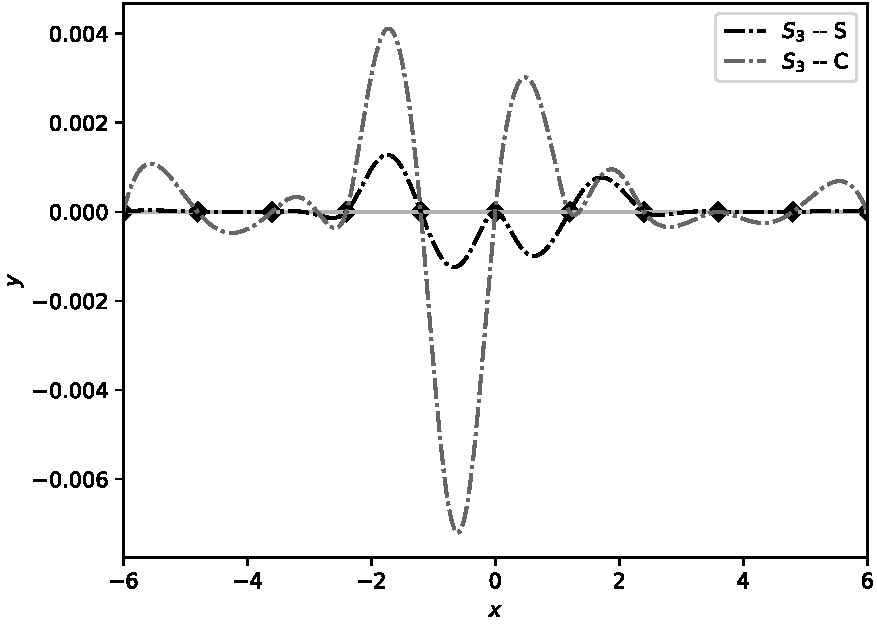
\includegraphics[width=.46\textwidth]{pictures/interpolate_spline_func1}} &
        \subcaptionbox{\centering Difference between interpolation and $f_2(x)\cdot g_2(x)$.}{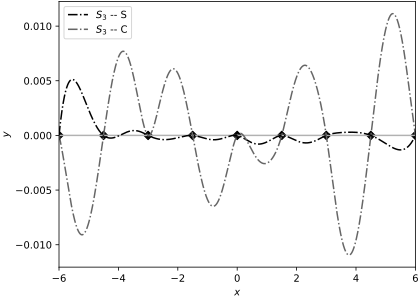
\includegraphics[width=.47\textwidth]{pictures/interpolate_spline_func2}}
    \end{tabular}
    \vspace{-.2em}
    \caption{In these figures $f_1(x) = 1/(1+x^2/10)$, $g_1(x) = 1/(1+(x+1)^2/10)$ and $f_2(x) = \cos(\sqrt{(x-1)^2/4+1})$, $g_2(x) = \sin(\sqrt{(x-2)^2/4+1})$. Interpolation was done on 11 and 9 samples points, respectively, by means of a separate interpolation method denoted by $S_3$ -- S and a combined interpolation method denoted by $S_3$ -- C.}
    \label{fig:res_2}
\end{figure}

\subsubsection{Calculating the integrals using the Newton-Cotes equations by interpolating $h_2(x)$}
We provide example calculations of using various Newton-Cotes equations to approximate the integral over $h_2(x)$, the general methods are presented in Section \ref{comb_interpol}.

The function values of $h_2(x)$ at the 9 samples points from Figure \ref{fig:res_1b} written in vector notation are:
\begin{equation}
    \scalemath{0.99}{
    \mathbf f =
    \begin{bmatrix}
        0.73018 & 0.24998 & -0.26794 & -0.02706 & 0.4321 & 0.44099 & 0.14023 & -0.43006 & -0.70876
    \end{bmatrix} \,.} \nonumber
\end{equation}
The value for $h$ can be calculated by dividing the total width of the interval by the total number of subintervals (which is one less than the number of sample points):
\begin{equation}
    h = \frac{12}{9-1} = \frac{3}{2} \,.\nonumber
\end{equation}
Now, for all different interpolating polynomials $N_1$, $N_2$, $N_{1-6-1}$, and $N_{2-6^*-2}$ we determine the corresponding vector from equation \ref{eq:vectors} (note that the coefficients can be found in equations \ref{eq:newton_cotes} and \ref{eq:6star}):
\begin{equation}
    \mathbf c_1 = \frac{3}{4}
    \begin{bmatrix}
        1 & 2 & 2 & 2 & 2 & 2 & 2 & 2 & 1
    \end{bmatrix} \,, \quad
    \mathbf c_2 = \frac{1}{2}
    \begin{bmatrix}
        1 & 4 & 2 & 4 & 2 & 4 & 2 & 4 & 1
    \end{bmatrix} \,,\nonumber
\end{equation}
\begin{equation}
    \mathbf c_{1-6-1} = \begin{bmatrix}
        \frac{3}{4} & \frac{3}{4} + \frac{3\cdot 41}{280} & \frac{3\cdot 216}{280} & \frac{3\cdot 27}{280} & \frac{3\cdot 272}{280} & \frac{3\cdot 27}{280} & \frac{3\cdot 216}{280} & \frac{3\cdot 41}{280} + \frac{3}{4} & \frac{3}{4}
    \end{bmatrix} \,,\nonumber
\end{equation}
\begin{equation}
    \mathbf c_{2-6^*-2} = \begin{bmatrix}
        \frac{1}{2} & 2 - \frac{3\cdot 4}{945} & \frac{1}{2}+\frac{3\cdot 171}{945} & \frac{3\cdot 612}{945} & \frac{3\cdot 332}{945} & \frac{3\cdot 612}{945} & \frac{3\cdot 171}{945}+\frac{1}{2} & -\frac{3\cdot 4}{945} + 2 & \frac{1}{2}
    \end{bmatrix} \,.\nonumber
\end{equation}
Now, we can finally approximate the integral by determining the integral over $N_1$, $N_2$, $N_{1-6-1}$, and $N_{2-6^*-2}$, this can thus be done without ever having to interpolate the function:
\begin{equation}
    \mathbf c_1 \mathbf f^\top \approx 0.823425 \,, \quad
    \mathbf c_2 \mathbf f^\top \approx 0.782800 \,, \quad
    \mathbf c_{1-6-1} \mathbf f^\top \approx 0.885348 \,, \quad
    \mathbf c_{2-6^*-2} \mathbf f^\top \approx 0.779280 \,. \nonumber
\end{equation}
Verifying the results in Table \ref{tab:res_1} and below.

\subsubsection{Calculating the integral over $f_2(x) \cdot g_2(x)$ using separate spline interpolation}
To replicate the results from Table \ref{tab:res_2} we first write $f_2(x)$ and $g_2(x)$ without subscripts, i.e. $f(x)$ and $g(x)$, to avoid confusion later on.
In this example we have used $n_f=3$ and $n_g = 5$.

To avoid rounding errors we modify the method in Section \ref{sep_interpol}, avoiding any high powers of $x_i$ when calculating the various values of $d_{ij}$.
The modification of the method is to shift all the subintervals $[x_i, x_{i+1}]$ to $[x_4, x_5] = [0, \frac{3}{2}]$ and carry out the interpolation for all the subintervals on this new domain.
Using this method we only need to calculate powers of $x_4=0$ and $x_5=\frac{3}{2}$ instead of powers of $x_i$ and $x_{i+1}$, this speeds up the process and avoids multiplying by large numbers resulting in less rounding errors in our answer.
For the shifted interpolation the coefficients of the interpolating polynomial of $f_3(x)$ (i.e. $\mathbf b_{3j}$) are now the coefficients after interpolating $f_3(x-\frac{3}{2})$ on the interval $[0, \frac{3}{2}]$.
Similarly, the coefficients for $\mathbf b_{1j}$ are the coefficients from interpolating $f_1(x-3\cdot \frac{3}{2})$ on the interval $[0, \frac{3}{2}]$.
To obtain the correct answer using these shifted interpolation coefficients we need to make a second adjustment to our method.
This is for calculating the values of $d_{ij}$ (equation \ref{eq:calc_dij}).
We need to use the values $x_4$ and $x_5$ repeatedly instead of $x_{i}$ and $x_{i+1}$, respectively.
Since $x_4=0$ this results in calculating and storing the values of $x_{5}^{j+k+1}/(j+k+1)$ for all values of $j+k$ before calculating (and storing if we have multiple sensors) the values of
\begin{equation}
    d_{ij} = \sum_{k=0}^{n_g} c_{ik} \frac{x_{5}^{j+k+1}}{j+k+1} \,. \nonumber
\end{equation}
All things considered, these modifications improve the accuracy of our results as they avoid rounding errors.

The function $f_3(x-\frac{3}{2})$ interpolated on $[x_4, x_5] = [0, \frac{3}{2}]$ is given as:
\begin{equation}
    f_3\left(x-\frac{3}{2}\right) \approx -0.02998 + 0.39005 x -0.03051 x^2 -0.014518 x^3 \,, \nonumber
\end{equation}
resulting in row $3$ of matrix $B$,
\begin{equation}
    \mathbf b_{3j} = \begin{bmatrix}-0.02998 & 0.39005 & -0.03051 & -0.014518 \end{bmatrix} \,. \nonumber \\
\end{equation}
Continuing this process to calculate all elements of $B$ and $C$ we can calculate the elements of $D$ and use equation \ref{eq:final_int} to approximate the integral.
In Appendix \ref{app:matrices} we listed all values of the matrices.
We note that the method seems like a lot of work, but after we initialize it we can easily calculate the sum in equation \ref{eq:final_int} again with a shift to approximate the integral for a different sensor.

Taking everything into account, using this method we get a value of $0.79902$ for the evaluation of the integral, which corresponds to an absolute difference of $0.00175$ and a relative difference of $0.219\%$.
Without the method of shifting the intervals we would have obtained the value $0.79958$ with a relative difference of $0.289\%$, due to rounding errors resulting from multiplying by a factor of $(x_{i+1}^{j+k+1} - x_i^{j+k+1})/(j+k+1)$.

The obtained value can be improved upon (by a tiny fraction) by increasing the order of the spline (or polynomial) used to interpolate $g(x)$, i.e. increasing $n_g$.
